\documentclass[1p]{elsarticle_modified}
%\bibliographystyle{elsarticle-num}

%\usepackage[colorlinks]{hyperref}
%\usepackage{abbrmath_seonhwa} %\Abb, \Ascr, \Acal ,\Abf, \Afrak
\usepackage{amsfonts}
\usepackage{amssymb}
\usepackage{amsmath}
\usepackage{amsthm}
\usepackage{scalefnt}
\usepackage{amsbsy}
\usepackage{kotex}
\usepackage{caption}
\usepackage{subfig}
\usepackage{color}
\usepackage{graphicx}
\usepackage{xcolor} %% white, black, red, green, blue, cyan, magenta, yellow
\usepackage{float}
\usepackage{setspace}
\usepackage{hyperref}

\usepackage{tikz}
\usetikzlibrary{arrows}

\usepackage{multirow}
\usepackage{array} % fixed length table
\usepackage{hhline}

%%%%%%%%%%%%%%%%%%%%%
\makeatletter
\renewcommand*\env@matrix[1][\arraystretch]{%
	\edef\arraystretch{#1}%
	\hskip -\arraycolsep
	\let\@ifnextchar\new@ifnextchar
	\array{*\c@MaxMatrixCols c}}
\makeatother %https://tex.stackexchange.com/questions/14071/how-can-i-increase-the-line-spacing-in-a-matrix
%%%%%%%%%%%%%%%

\usepackage[normalem]{ulem}

\newcommand{\msout}[1]{\ifmmode\text{\sout{\ensuremath{#1}}}\else\sout{#1}\fi}
%SOURCE: \msout is \stkout macro in https://tex.stackexchange.com/questions/20609/strikeout-in-math-mode

\newcommand{\cancel}[1]{
	\ifmmode
	{\color{red}\msout{#1}}
	\else
	{\color{red}\sout{#1}}
	\fi
}

\newcommand{\add}[1]{
	{\color{blue}\uwave{#1}}
}

\newcommand{\replace}[2]{
	\ifmmode
	{\color{red}\msout{#1}}{\color{blue}\uwave{#2}}
	\else
	{\color{red}\sout{#1}}{\color{blue}\uwave{#2}}
	\fi
}

\newcommand{\Sol}{\mathcal{S}} %segment
\newcommand{\D}{D} %diagram
\newcommand{\A}{\mathcal{A}} %arc


%%%%%%%%%%%%%%%%%%%%%%%%%%%%%5 test

\def\sl{\operatorname{\textup{SL}}(2,\Cbb)}
\def\psl{\operatorname{\textup{PSL}}(2,\Cbb)}
\def\quan{\mkern 1mu \triangleright \mkern 1mu}

\theoremstyle{definition}
\newtheorem{thm}{Theorem}[section]
\newtheorem{prop}[thm]{Proposition}
\newtheorem{lem}[thm]{Lemma}
\newtheorem{ques}[thm]{Question}
\newtheorem{cor}[thm]{Corollary}
\newtheorem{defn}[thm]{Definition}
\newtheorem{exam}[thm]{Example}
\newtheorem{rmk}[thm]{Remark}
\newtheorem{alg}[thm]{Algorithm}

\newcommand{\I}{\sqrt{-1}}
\begin{document}

%\begin{frontmatter}
%
%\title{Boundary parabolic representations of knots up to 8 crossings}
%
%%% Group authors per affiliation:
%\author{Yunhi Cho} 
%\address{Department of Mathematics, University of Seoul, Seoul, Korea}
%\ead{yhcho@uos.ac.kr}
%
%
%\author{Seonhwa Kim} %\fnref{s_kim}}
%\address{Center for Geometry and Physics, Institute for Basic Science, Pohang, 37673, Korea}
%\ead{ryeona17@ibs.re.kr}
%
%\author{Hyuk Kim}
%\address{Department of Mathematical Sciences, Seoul National University, Seoul 08826, Korea}
%\ead{hyukkim@snu.ac.kr}
%
%\author{Seokbeom Yoon}
%\address{Department of Mathematical Sciences, Seoul National University, Seoul, 08826,  Korea}
%\ead{sbyoon15@snu.ac.kr}
%
%\begin{abstract}
%We find all boundary parabolic representation of knots up to 8 crossings.
%
%\end{abstract}
%\begin{keyword}
%    \MSC[2010] 57M25 
%\end{keyword}
%
%\end{frontmatter}

%\linenumbers
%\tableofcontents
%
\newcommand\colored[1]{\textcolor{white}{\rule[-0.35ex]{0.8em}{1.4ex}}\kern-0.8em\color{red} #1}%
%\newcommand\colored[1]{\textcolor{white}{ #1}\kern-2.17ex	\textcolor{white}{ #1}\kern-1.81ex	\textcolor{white}{ #1}\kern-2.15ex\color{red}#1	}

{\Large $\underline{12a_{0881}~(K12a_{0881})}$}

\setlength{\tabcolsep}{10pt}
\renewcommand{\arraystretch}{1.6}
\vspace{1cm}\begin{tabular}{m{100pt}>{\centering\arraybackslash}m{274pt}}
\multirow{5}{120pt}{
	\centering
	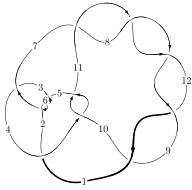
\includegraphics[width=112pt]{../../../GIT/diagram.site/Diagrams/png/1682_12a_0881.png}\\
\ \ \ A knot diagram\footnotemark}&
\allowdisplaybreaks
\textbf{Linearized knot diagam} \\
\cline{2-2}
 &
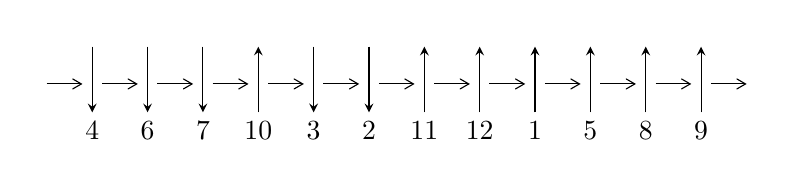
\begin{tikzpicture}[x=20pt, y=17pt]
	% nodes
	\node (C0) at (0, 0) {};
	\node (C1) at (1, 0) {};
	\node (C1U) at (1, +1) {};
	\node (C1D) at (1, -1) {4};

	\node (C2) at (2, 0) {};
	\node (C2U) at (2, +1) {};
	\node (C2D) at (2, -1) {6};

	\node (C3) at (3, 0) {};
	\node (C3U) at (3, +1) {};
	\node (C3D) at (3, -1) {7};

	\node (C4) at (4, 0) {};
	\node (C4U) at (4, +1) {};
	\node (C4D) at (4, -1) {10};

	\node (C5) at (5, 0) {};
	\node (C5U) at (5, +1) {};
	\node (C5D) at (5, -1) {3};

	\node (C6) at (6, 0) {};
	\node (C6U) at (6, +1) {};
	\node (C6D) at (6, -1) {2};

	\node (C7) at (7, 0) {};
	\node (C7U) at (7, +1) {};
	\node (C7D) at (7, -1) {11};

	\node (C8) at (8, 0) {};
	\node (C8U) at (8, +1) {};
	\node (C8D) at (8, -1) {12};

	\node (C9) at (9, 0) {};
	\node (C9U) at (9, +1) {};
	\node (C9D) at (9, -1) {1};

	\node (C10) at (10, 0) {};
	\node (C10U) at (10, +1) {};
	\node (C10D) at (10, -1) {5};

	\node (C11) at (11, 0) {};
	\node (C11U) at (11, +1) {};
	\node (C11D) at (11, -1) {8};

	\node (C12) at (12, 0) {};
	\node (C12U) at (12, +1) {};
	\node (C12D) at (12, -1) {9};
	\node (C13) at (13, 0) {};

	% arrows
	\draw[->,>={angle 60}]
	(C0) edge (C1) (C1) edge (C2) (C2) edge (C3) (C3) edge (C4) (C4) edge (C5) (C5) edge (C6) (C6) edge (C7) (C7) edge (C8) (C8) edge (C9) (C9) edge (C10) (C10) edge (C11) (C11) edge (C12) (C12) edge (C13) ;	\draw[->,>=stealth]
	(C1U) edge (C1D) (C2U) edge (C2D) (C3U) edge (C3D) (C4D) edge (C4U) (C5U) edge (C5D) (C6U) edge (C6D) (C7D) edge (C7U) (C8D) edge (C8U) (C9D) edge (C9U) (C10D) edge (C10U) (C11D) edge (C11U) (C12D) edge (C12U) ;
	\end{tikzpicture} \\
\hhline{~~} \\& 
\textbf{Solving Sequence} \\ \cline{2-2} 
 &
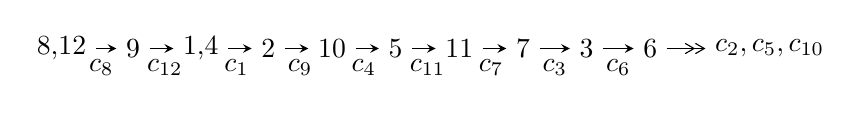
\begin{tikzpicture}[x=23pt, y=7pt]
	% node
	\node (A0) at (-1/8, 0) {8,12};
	\node (A1) at (1, 0) {9};
	\node (A2) at (33/16, 0) {1,4};
	\node (A3) at (25/8, 0) {2};
	\node (A4) at (33/8, 0) {10};
	\node (A5) at (41/8, 0) {5};
	\node (A6) at (49/8, 0) {11};
	\node (A7) at (57/8, 0) {7};
	\node (A8) at (65/8, 0) {3};
	\node (A9) at (73/8, 0) {6};
	\node (C1) at (1/2, -1) {$c_{8}$};
	\node (C2) at (3/2, -1) {$c_{12}$};
	\node (C3) at (21/8, -1) {$c_{1}$};
	\node (C4) at (29/8, -1) {$c_{9}$};
	\node (C5) at (37/8, -1) {$c_{4}$};
	\node (C6) at (45/8, -1) {$c_{11}$};
	\node (C7) at (53/8, -1) {$c_{7}$};
	\node (C8) at (61/8, -1) {$c_{3}$};
	\node (C9) at (69/8, -1) {$c_{6}$};
	\node (A10) at (11, 0) {$c_{2},c_{5},c_{10}$};

	% edge
	\draw[->,>=stealth]	
	(A0) edge (A1) (A1) edge (A2) (A2) edge (A3) (A3) edge (A4) (A4) edge (A5) (A5) edge (A6) (A6) edge (A7) (A7) edge (A8) (A8) edge (A9) ;
	\draw[->>,>={angle 60}]	
	(A9) edge (A10);
\end{tikzpicture} \\ 

\end{tabular} \\

\footnotetext{
The image of knot diagram is generated by the software ``\textbf{Draw programme}" developed by Andrew Bartholomew(\url{http://www.layer8.co.uk/maths/draw/index.htm\#Running-draw}), where we modified some parts for our purpose(\url{https://github.com/CATsTAILs/LinksPainter}).
}\phantom \\ \newline 
\centering \textbf{Ideals for irreducible components\footnotemark of $X_{\text{par}}$} 
 
\begin{align*}
I^u_{1}&=\langle 
30 u^{49}+63 u^{48}+\cdots+4 b+19,\;7 u^{48}+15 u^{47}+\cdots+4 a-3,\;u^{50}+4 u^{49}+\cdots- u+1\rangle \\
I^u_{2}&=\langle 
b+a,\;a^3+a^2-1,\;u^2- u-1\rangle \\
\\
\end{align*}
\raggedright * 2 irreducible components of $\dim_{\mathbb{C}}=0$, with total 56 representations.\\
\footnotetext{All coefficients of polynomials are rational numbers. But the coefficients are sometimes approximated in decimal forms when there is not enough margin.}
\newpage
\renewcommand{\arraystretch}{1}
\centering \section*{I. $I^u_{1}= \langle 30 u^{49}+63 u^{48}+\cdots+4 b+19,\;7 u^{48}+15 u^{47}+\cdots+4 a-3,\;u^{50}+4 u^{49}+\cdots- u+1 \rangle$}
\flushleft \textbf{(i) Arc colorings}\\
\begin{tabular}{m{7pt} m{180pt} m{7pt} m{180pt} }
\flushright $a_{8}=$&$\begin{pmatrix}1\\0\end{pmatrix}$ \\
\flushright $a_{12}=$&$\begin{pmatrix}0\\u\end{pmatrix}$ \\
\flushright $a_{9}=$&$\begin{pmatrix}1\\- u^2\end{pmatrix}$ \\
\flushright $a_{1}=$&$\begin{pmatrix}u\\- u^3+u\end{pmatrix}$ \\
\flushright $a_{4}=$&$\begin{pmatrix}-\frac{7}{4} u^{48}-\frac{15}{4} u^{47}+\cdots-\frac{7}{2} u+\frac{3}{4}\\-\frac{15}{2} u^{49}-\frac{63}{4} u^{48}+\cdots+6 u-\frac{19}{4}\end{pmatrix}$ \\
\flushright $a_{2}=$&$\begin{pmatrix}\frac{1}{4} u^{49}+\frac{3}{4} u^{48}+\cdots+\frac{23}{4} u+1\\-\frac{1}{4} u^{49}-\frac{3}{4} u^{48}+\cdots-5 u^2+\frac{1}{4} u\end{pmatrix}$ \\
\flushright $a_{10}=$&$\begin{pmatrix}- u^2+1\\u^4-2 u^2\end{pmatrix}$ \\
\flushright $a_{5}=$&$\begin{pmatrix}-20 u^{49}-\frac{185}{4} u^{48}+\cdots+\frac{29}{2} u-\frac{43}{4}\\\frac{51}{2} u^{49}+\frac{235}{4} u^{48}+\cdots-23 u+\frac{55}{4}\end{pmatrix}$ \\
\flushright $a_{11}=$&$\begin{pmatrix}- u\\u\end{pmatrix}$ \\
\flushright $a_{7}=$&$\begin{pmatrix}- u^2+1\\u^2\end{pmatrix}$ \\
\flushright $a_{3}=$&$\begin{pmatrix}-\frac{111}{4} u^{49}-65 u^{48}+\cdots+\frac{85}{4} u-\frac{63}{4}\\34.7500 u^{49}+81.2500 u^{48}+\cdots-32.7500 u+19.5000\end{pmatrix}$ \\
\flushright $a_{6}=$&$\begin{pmatrix}-\frac{9}{2} u^{49}-\frac{21}{2} u^{48}+\cdots+4 u-2\\\frac{21}{4} u^{49}+\frac{51}{4} u^{48}+\cdots-\frac{19}{4} u+3\end{pmatrix}$\\&\end{tabular}
\flushleft \textbf{(ii) Obstruction class $= -1$}\\~\\
\flushleft \textbf{(iii) Cusp Shapes $= 25 u^{49}+59 u^{48}+\cdots-\frac{83}{2} u+\frac{25}{2}$}\\~\\
\newpage\renewcommand{\arraystretch}{1}
\flushleft \textbf{(iv) u-Polynomials at the component}\newline \\
\begin{tabular}{m{50pt}|m{274pt}}
Crossings & \hspace{64pt}u-Polynomials at each crossing \\
\hline $$\begin{aligned}c_{1}\end{aligned}$$&$\begin{aligned}
&u^{50}-9 u^{49}+\cdots+1832 u+113
\end{aligned}$\\
\hline $$\begin{aligned}c_{2},c_{5},c_{6}\end{aligned}$$&$\begin{aligned}
&u^{50}-3 u^{49}+\cdots-10 u+1
\end{aligned}$\\
\hline $$\begin{aligned}c_{3}\end{aligned}$$&$\begin{aligned}
&u^{50}+3 u^{49}+\cdots-2392 u+241
\end{aligned}$\\
\hline $$\begin{aligned}c_{4},c_{10}\end{aligned}$$&$\begin{aligned}
&u^{50}- u^{49}+\cdots-96 u+64
\end{aligned}$\\
\hline $$\begin{aligned}c_{7},c_{8},c_{9}\\c_{11},c_{12}\end{aligned}$$&$\begin{aligned}
&u^{50}-4 u^{49}+\cdots+u+1
\end{aligned}$\\
\hline
\end{tabular}\\~\\
\newpage\renewcommand{\arraystretch}{1}
\flushleft \textbf{(v) Riley Polynomials at the component}\newline \\
\begin{tabular}{m{50pt}|m{274pt}}
Crossings & \hspace{64pt}Riley Polynomials at each crossing \\
\hline $$\begin{aligned}c_{1}\end{aligned}$$&$\begin{aligned}
&y^{50}+31 y^{49}+\cdots-5984830 y+12769
\end{aligned}$\\
\hline $$\begin{aligned}c_{2},c_{5},c_{6}\end{aligned}$$&$\begin{aligned}
&y^{50}+47 y^{49}+\cdots-54 y+1
\end{aligned}$\\
\hline $$\begin{aligned}c_{3}\end{aligned}$$&$\begin{aligned}
&y^{50}+11 y^{49}+\cdots-2239214 y+58081
\end{aligned}$\\
\hline $$\begin{aligned}c_{4},c_{10}\end{aligned}$$&$\begin{aligned}
&y^{50}-35 y^{49}+\cdots-54272 y+4096
\end{aligned}$\\
\hline $$\begin{aligned}c_{7},c_{8},c_{9}\\c_{11},c_{12}\end{aligned}$$&$\begin{aligned}
&y^{50}-68 y^{49}+\cdots+9 y+1
\end{aligned}$\\
\hline
\end{tabular}\\~\\
\newpage\flushleft \textbf{(vi) Complex Volumes and Cusp Shapes}
$$\begin{array}{c|c|c}  
\text{Solutions to }I^u_{1}& \I (\text{vol} + \sqrt{-1}CS) & \text{Cusp shape}\\
 \hline 
\begin{aligned}
u &= -0.952202 + 0.085743 I \\
a &= \phantom{-}0.263868 + 0.811802 I \\
b &= \phantom{-}0.109466 + 1.005260 I\end{aligned}
 & \phantom{-}1.99660 - 1.56126 I & \phantom{-0.000000 -}0. + 4.54210 I \\ \hline\begin{aligned}
u &= -0.952202 - 0.085743 I \\
a &= \phantom{-}0.263868 - 0.811802 I \\
b &= \phantom{-}0.109466 - 1.005260 I\end{aligned}
 & \phantom{-}1.99660 + 1.56126 I & \phantom{-0.000000 } 0. - 4.54210 I \\ \hline\begin{aligned}
u &= -1.051590 + 0.116393 I \\
a &= -0.460087 - 1.130740 I \\
b &= \phantom{-}0.029530 - 1.139970 I\end{aligned}
 & \phantom{-}7.55680 - 4.35419 I & \phantom{-0.000000 } 0 \\ \hline\begin{aligned}
u &= -1.051590 - 0.116393 I \\
a &= -0.460087 + 1.130740 I \\
b &= \phantom{-}0.029530 + 1.139970 I\end{aligned}
 & \phantom{-}7.55680 + 4.35419 I & \phantom{-0.000000 } 0 \\ \hline\begin{aligned}
u &= \phantom{-}0.926369 + 0.110294 I \\
a &= -0.951862 + 0.190261 I \\
b &= \phantom{-}1.207080 - 0.506059 I\end{aligned}
 & \phantom{-}4.83990 + 3.67287 I & \phantom{-}11.52712 - 5.42395 I \\ \hline\begin{aligned}
u &= \phantom{-}0.926369 - 0.110294 I \\
a &= -0.951862 - 0.190261 I \\
b &= \phantom{-}1.207080 + 0.506059 I\end{aligned}
 & \phantom{-}4.83990 - 3.67287 I & \phantom{-}11.52712 + 5.42395 I \\ \hline\begin{aligned}
u &= \phantom{-}0.926358\phantom{ +0.000000I} \\
a &= \phantom{-}1.08741\phantom{ +0.000000I} \\
b &= -1.30017\phantom{ +0.000000I}\end{aligned}
 & \phantom{-}1.12359\phantom{ +0.000000I} & \phantom{-}7.78030\phantom{ +0.000000I} \\ \hline\begin{aligned}
u &= \phantom{-}1.075460 + 0.335893 I \\
a &= \phantom{-}0.318078 + 0.440056 I \\
b &= \phantom{-}0.173538 + 1.100140 I\end{aligned}
 & \phantom{-}5.70451 + 6.74184 I & \phantom{-0.000000 } 0 \\ \hline\begin{aligned}
u &= \phantom{-}1.075460 - 0.335893 I \\
a &= \phantom{-}0.318078 - 0.440056 I \\
b &= \phantom{-}0.173538 - 1.100140 I\end{aligned}
 & \phantom{-}5.70451 - 6.74184 I & \phantom{-0.000000 } 0 \\ \hline\begin{aligned}
u &= \phantom{-}1.101720 + 0.265116 I \\
a &= -0.631574 - 0.369790 I \\
b &= \phantom{-}0.069190 - 0.623696 I\end{aligned}
 & \phantom{-}6.52824 + 2.59024 I & \phantom{-0.000000 } 0\\
 \hline 
 \end{array}$$\newpage$$\begin{array}{c|c|c}  
\text{Solutions to }I^u_{1}& \I (\text{vol} + \sqrt{-1}CS) & \text{Cusp shape}\\
 \hline 
\begin{aligned}
u &= \phantom{-}1.101720 - 0.265116 I \\
a &= -0.631574 + 0.369790 I \\
b &= \phantom{-}0.069190 + 0.623696 I\end{aligned}
 & \phantom{-}6.52824 - 2.59024 I & \phantom{-0.000000 } 0 \\ \hline\begin{aligned}
u &= \phantom{-}1.091080 + 0.380456 I \\
a &= -0.163597 - 0.625898 I \\
b &= -0.536851 - 1.297450 I\end{aligned}
 & \phantom{-}11.5454 + 10.2862 I & \phantom{-0.000000 } 0 \\ \hline\begin{aligned}
u &= \phantom{-}1.091080 - 0.380456 I \\
a &= -0.163597 + 0.625898 I \\
b &= -0.536851 + 1.297450 I\end{aligned}
 & \phantom{-}11.5454 - 10.2862 I & \phantom{-0.000000 } 0 \\ \hline\begin{aligned}
u &= -0.740193 + 0.295777 I \\
a &= -0.361219 - 0.137662 I \\
b &= -0.870973 - 0.536080 I\end{aligned}
 & \phantom{-}4.15678 - 0.49764 I & \phantom{-}9.03893 + 1.33769 I \\ \hline\begin{aligned}
u &= -0.740193 - 0.295777 I \\
a &= -0.361219 + 0.137662 I \\
b &= -0.870973 + 0.536080 I\end{aligned}
 & \phantom{-}4.15678 + 0.49764 I & \phantom{-}9.03893 - 1.33769 I \\ \hline\begin{aligned}
u &= \phantom{-}1.199130 + 0.267015 I \\
a &= \phantom{-}0.903623 + 0.631411 I \\
b &= \phantom{-}0.208467 + 0.051458 I\end{aligned}
 & \phantom{-}13.08760 + 0.25307 I & \phantom{-0.000000 } 0 \\ \hline\begin{aligned}
u &= \phantom{-}1.199130 - 0.267015 I \\
a &= \phantom{-}0.903623 - 0.631411 I \\
b &= \phantom{-}0.208467 - 0.051458 I\end{aligned}
 & \phantom{-}13.08760 - 0.25307 I & \phantom{-0.000000 } 0 \\ \hline\begin{aligned}
u &= -0.470779 + 0.592707 I \\
a &= \phantom{-}0.805640 - 0.073631 I \\
b &= -0.525112 + 1.088250 I\end{aligned}
 & \phantom{-}7.73029 + 2.70190 I & \phantom{-}9.92902 - 0.03562 I \\ \hline\begin{aligned}
u &= -0.470779 - 0.592707 I \\
a &= \phantom{-}0.805640 + 0.073631 I \\
b &= -0.525112 - 1.088250 I\end{aligned}
 & \phantom{-}7.73029 - 2.70190 I & \phantom{-}9.92902 + 0.03562 I \\ \hline\begin{aligned}
u &= -0.301413 + 0.651199 I \\
a &= -1.27352 + 0.89636 I \\
b &= -0.537119 - 0.669077 I\end{aligned}
 & \phantom{-}7.21081 - 6.77625 I & \phantom{-}8.31083 + 6.21335 I\\
 \hline 
 \end{array}$$\newpage$$\begin{array}{c|c|c}  
\text{Solutions to }I^u_{1}& \I (\text{vol} + \sqrt{-1}CS) & \text{Cusp shape}\\
 \hline 
\begin{aligned}
u &= -0.301413 - 0.651199 I \\
a &= -1.27352 - 0.89636 I \\
b &= -0.537119 + 0.669077 I\end{aligned}
 & \phantom{-}7.21081 + 6.77625 I & \phantom{-}8.31083 - 6.21335 I \\ \hline\begin{aligned}
u &= -0.295790 + 0.583078 I \\
a &= \phantom{-}0.912564 - 0.926539 I \\
b &= \phantom{-}0.190072 + 0.467950 I\end{aligned}
 & \phantom{-}1.43056 - 3.60804 I & \phantom{-}4.24958 + 7.07743 I \\ \hline\begin{aligned}
u &= -0.295790 - 0.583078 I \\
a &= \phantom{-}0.912564 + 0.926539 I \\
b &= \phantom{-}0.190072 - 0.467950 I\end{aligned}
 & \phantom{-}1.43056 + 3.60804 I & \phantom{-}4.24958 - 7.07743 I \\ \hline\begin{aligned}
u &= -0.405535 + 0.509845 I \\
a &= -0.537103 + 0.460008 I \\
b &= \phantom{-}0.355378 - 0.582565 I\end{aligned}
 & \phantom{-}1.81710 + 0.00783 I & \phantom{-}6.28682 + 0.01976 I \\ \hline\begin{aligned}
u &= -0.405535 - 0.509845 I \\
a &= -0.537103 - 0.460008 I \\
b &= \phantom{-}0.355378 + 0.582565 I\end{aligned}
 & \phantom{-}1.81710 - 0.00783 I & \phantom{-}6.28682 - 0.01976 I \\ \hline\begin{aligned}
u &= -0.512306\phantom{ +0.000000I} \\
a &= \phantom{-}0.313006\phantom{ +0.000000I} \\
b &= \phantom{-}0.321368\phantom{ +0.000000I}\end{aligned}
 & \phantom{-}0.766149\phantom{ +0.000000I} & \phantom{-}13.4410\phantom{ +0.000000I} \\ \hline\begin{aligned}
u &= -0.033821 + 0.416681 I \\
a &= -0.02102 + 1.94574 I \\
b &= \phantom{-}0.405990 + 0.159838 I\end{aligned}
 & \phantom{-}2.06372 - 1.98561 I & \phantom{-}1.75080 + 4.13320 I \\ \hline\begin{aligned}
u &= -0.033821 - 0.416681 I \\
a &= -0.02102 - 1.94574 I \\
b &= \phantom{-}0.405990 - 0.159838 I\end{aligned}
 & \phantom{-}2.06372 + 1.98561 I & \phantom{-}1.75080 - 4.13320 I \\ \hline\begin{aligned}
u &= \phantom{-}1.59708\phantom{ +0.000000I} \\
a &= -0.845107\phantom{ +0.000000I} \\
b &= \phantom{-}1.07699\phantom{ +0.000000I}\end{aligned}
 & \phantom{-}8.19154\phantom{ +0.000000I} & \phantom{-0.000000 } 0 \\ \hline\begin{aligned}
u &= \phantom{-}1.61144 + 0.05910 I \\
a &= \phantom{-}1.25524 - 0.79623 I \\
b &= -1.80165 + 0.80672 I\end{aligned}
 & \phantom{-}12.23120 + 1.76270 I & \phantom{-0.000000 } 0\\
 \hline 
 \end{array}$$\newpage$$\begin{array}{c|c|c}  
\text{Solutions to }I^u_{1}& \I (\text{vol} + \sqrt{-1}CS) & \text{Cusp shape}\\
 \hline 
\begin{aligned}
u &= \phantom{-}1.61144 - 0.05910 I \\
a &= \phantom{-}1.25524 + 0.79623 I \\
b &= -1.80165 - 0.80672 I\end{aligned}
 & \phantom{-}12.23120 - 1.76270 I & \phantom{-0.000000 } 0 \\ \hline\begin{aligned}
u &= \phantom{-}0.267156 + 0.194860 I \\
a &= \phantom{-}0.14623 + 2.75307 I \\
b &= \phantom{-}0.727620 - 0.740672 I\end{aligned}
 & \phantom{-}3.42049 + 3.22954 I & -0.37490 - 5.13369 I \\ \hline\begin{aligned}
u &= \phantom{-}0.267156 - 0.194860 I \\
a &= \phantom{-}0.14623 - 2.75307 I \\
b &= \phantom{-}0.727620 + 0.740672 I\end{aligned}
 & \phantom{-}3.42049 - 3.22954 I & -0.37490 + 5.13369 I \\ \hline\begin{aligned}
u &= -1.71592\phantom{ +0.000000I} \\
a &= \phantom{-}0.726622\phantom{ +0.000000I} \\
b &= -0.423053\phantom{ +0.000000I}\end{aligned}
 & \phantom{-}10.6526\phantom{ +0.000000I} & \phantom{-0.000000 } 0 \\ \hline\begin{aligned}
u &= -1.71698 + 0.02280 I \\
a &= -0.638945 - 0.755487 I \\
b &= \phantom{-}0.367724 + 1.082380 I\end{aligned}
 & \phantom{-}14.3705 - 4.1609 I & \phantom{-0.000000 } 0 \\ \hline\begin{aligned}
u &= -1.71698 - 0.02280 I \\
a &= -0.638945 + 0.755487 I \\
b &= \phantom{-}0.367724 - 1.082380 I\end{aligned}
 & \phantom{-}14.3705 + 4.1609 I & \phantom{-0.000000 } 0 \\ \hline\begin{aligned}
u &= \phantom{-}1.71834 + 0.01659 I \\
a &= -0.32264 + 2.56462 I \\
b &= \phantom{-}0.69393 - 4.29665 I\end{aligned}
 & \phantom{-}11.59990 + 1.93326 I & \phantom{-0.000000 } 0 \\ \hline\begin{aligned}
u &= \phantom{-}1.71834 - 0.01659 I \\
a &= -0.32264 - 2.56462 I \\
b &= \phantom{-}0.69393 + 4.29665 I\end{aligned}
 & \phantom{-}11.59990 - 1.93326 I & \phantom{-0.000000 } 0 \\ \hline\begin{aligned}
u &= \phantom{-}1.74020 + 0.02935 I \\
a &= \phantom{-}0.58408 - 2.98539 I \\
b &= -1.34410 + 5.19321 I\end{aligned}
 & \phantom{-}17.6233 + 4.9552 I & \phantom{-0.000000 } 0 \\ \hline\begin{aligned}
u &= \phantom{-}1.74020 - 0.02935 I \\
a &= \phantom{-}0.58408 + 2.98539 I \\
b &= -1.34410 - 5.19321 I\end{aligned}
 & \phantom{-}17.6233 - 4.9552 I & \phantom{-0.000000 } 0\\
 \hline 
 \end{array}$$\newpage$$\begin{array}{c|c|c}  
\text{Solutions to }I^u_{1}& \I (\text{vol} + \sqrt{-1}CS) & \text{Cusp shape}\\
 \hline 
\begin{aligned}
u &= \phantom{-}0.102654 + 0.234461 I \\
a &= -0.48752 - 2.52124 I \\
b &= -0.550472 + 0.258801 I\end{aligned}
 & -1.186530 + 0.460043 I & -6.06013 - 1.97452 I \\ \hline\begin{aligned}
u &= \phantom{-}0.102654 - 0.234461 I \\
a &= -0.48752 + 2.52124 I \\
b &= -0.550472 - 0.258801 I\end{aligned}
 & -1.186530 - 0.460043 I & -6.06013 + 1.97452 I \\ \hline\begin{aligned}
u &= -1.74331 + 0.08919 I \\
a &= -0.36769 + 2.41491 I \\
b &= \phantom{-}0.37187 - 4.07506 I\end{aligned}
 & \phantom{-}15.7539 - 8.5170 I & \phantom{-0.000000 } 0 \\ \hline\begin{aligned}
u &= -1.74331 - 0.08919 I \\
a &= -0.36769 - 2.41491 I \\
b &= \phantom{-}0.37187 + 4.07506 I\end{aligned}
 & \phantom{-}15.7539 + 8.5170 I & \phantom{-0.000000 } 0 \\ \hline\begin{aligned}
u &= -1.74805 + 0.07009 I \\
a &= \phantom{-}0.42579 - 1.94514 I \\
b &= -0.80402 + 3.33285 I\end{aligned}
 & \phantom{-}16.7378 - 4.0067 I & \phantom{-0.000000 } 0 \\ \hline\begin{aligned}
u &= -1.74805 - 0.07009 I \\
a &= \phantom{-}0.42579 + 1.94514 I \\
b &= -0.80402 - 3.33285 I\end{aligned}
 & \phantom{-}16.7378 + 4.0067 I & \phantom{-0.000000 } 0 \\ \hline\begin{aligned}
u &= -1.74828 + 0.10270 I \\
a &= \phantom{-}0.50895 - 2.70608 I \\
b &= -0.35501 + 4.68791 I\end{aligned}
 & -17.8318 - 12.3199 I & \phantom{-0.000000 } 0 \\ \hline\begin{aligned}
u &= -1.74828 - 0.10270 I \\
a &= \phantom{-}0.50895 + 2.70608 I \\
b &= -0.35501 - 4.68791 I\end{aligned}
 & -17.8318 + 12.3199 I & \phantom{-0.000000 } 0 \\ \hline\begin{aligned}
u &= -1.77321 + 0.06163 I \\
a &= -1.04826 + 1.68240 I \\
b &= \phantom{-}2.07789 - 3.22013 I\end{aligned}
 & -15.6447 - 1.6429 I & \phantom{-0.000000 } 0 \\ \hline\begin{aligned}
u &= -1.77321 - 0.06163 I \\
a &= -1.04826 - 1.68240 I \\
b &= \phantom{-}2.07789 + 3.22013 I\end{aligned}
 & -15.6447 + 1.6429 I & \phantom{-0.000000 } 0\\
 \hline 
 \end{array}$$\newpage\newpage\renewcommand{\arraystretch}{1}
\centering \section*{II. $I^u_{2}= \langle b+a,\;a^3+a^2-1,\;u^2- u-1 \rangle$}
\flushleft \textbf{(i) Arc colorings}\\
\begin{tabular}{m{7pt} m{180pt} m{7pt} m{180pt} }
\flushright $a_{8}=$&$\begin{pmatrix}1\\0\end{pmatrix}$ \\
\flushright $a_{12}=$&$\begin{pmatrix}0\\u\end{pmatrix}$ \\
\flushright $a_{9}=$&$\begin{pmatrix}1\\- u-1\end{pmatrix}$ \\
\flushright $a_{1}=$&$\begin{pmatrix}u\\- u-1\end{pmatrix}$ \\
\flushright $a_{4}=$&$\begin{pmatrix}a\\- a\end{pmatrix}$ \\
\flushright $a_{2}=$&$\begin{pmatrix}a^2+u\\- a^2- u-1\end{pmatrix}$ \\
\flushright $a_{10}=$&$\begin{pmatrix}- u\\u\end{pmatrix}$ \\
\flushright $a_{5}=$&$\begin{pmatrix}a\\- a\end{pmatrix}$ \\
\flushright $a_{11}=$&$\begin{pmatrix}- u\\u\end{pmatrix}$ \\
\flushright $a_{7}=$&$\begin{pmatrix}- u\\u+1\end{pmatrix}$ \\
\flushright $a_{3}=$&$\begin{pmatrix}a u+a\\- a u-2 a\end{pmatrix}$ \\
\flushright $a_{6}=$&$\begin{pmatrix}a^2 u+a^2+a- u-1\\- a^2 u-2 a^2- a+u+2\end{pmatrix}$\\&\end{tabular}
\flushleft \textbf{(ii) Obstruction class $= 1$}\\~\\
\flushleft \textbf{(iii) Cusp Shapes $= a^2 u-2 a^2- a u-5 a- u+5$}\\~\\
\newpage\renewcommand{\arraystretch}{1}
\flushleft \textbf{(iv) u-Polynomials at the component}\newline \\
\begin{tabular}{m{50pt}|m{274pt}}
Crossings & \hspace{64pt}u-Polynomials at each crossing \\
\hline $$\begin{aligned}c_{1},c_{3}\end{aligned}$$&$\begin{aligned}
&(u^3+u^2-1)^2
\end{aligned}$\\
\hline $$\begin{aligned}c_{2}\end{aligned}$$&$\begin{aligned}
&(u^3- u^2+2 u-1)^2
\end{aligned}$\\
\hline $$\begin{aligned}c_{4},c_{10}\end{aligned}$$&$\begin{aligned}
&u^6
\end{aligned}$\\
\hline $$\begin{aligned}c_{5},c_{6}\end{aligned}$$&$\begin{aligned}
&(u^3+u^2+2 u+1)^2
\end{aligned}$\\
\hline $$\begin{aligned}c_{7},c_{8},c_{9}\end{aligned}$$&$\begin{aligned}
&(u^2- u-1)^3
\end{aligned}$\\
\hline $$\begin{aligned}c_{11},c_{12}\end{aligned}$$&$\begin{aligned}
&(u^2+u-1)^3
\end{aligned}$\\
\hline
\end{tabular}\\~\\
\newpage\renewcommand{\arraystretch}{1}
\flushleft \textbf{(v) Riley Polynomials at the component}\newline \\
\begin{tabular}{m{50pt}|m{274pt}}
Crossings & \hspace{64pt}Riley Polynomials at each crossing \\
\hline $$\begin{aligned}c_{1},c_{3}\end{aligned}$$&$\begin{aligned}
&(y^3- y^2+2 y-1)^2
\end{aligned}$\\
\hline $$\begin{aligned}c_{2},c_{5},c_{6}\end{aligned}$$&$\begin{aligned}
&(y^3+3 y^2+2 y-1)^2
\end{aligned}$\\
\hline $$\begin{aligned}c_{4},c_{10}\end{aligned}$$&$\begin{aligned}
&y^6
\end{aligned}$\\
\hline $$\begin{aligned}c_{7},c_{8},c_{9}\\c_{11},c_{12}\end{aligned}$$&$\begin{aligned}
&(y^2-3 y+1)^3
\end{aligned}$\\
\hline
\end{tabular}\\~\\
\newpage\flushleft \textbf{(vi) Complex Volumes and Cusp Shapes}
$$\begin{array}{c|c|c}  
\text{Solutions to }I^u_{2}& \I (\text{vol} + \sqrt{-1}CS) & \text{Cusp shape}\\
 \hline 
\begin{aligned}
u &= -0.618034\phantom{ +0.000000I} \\
a &= -0.877439 + 0.744862 I \\
b &= \phantom{-}0.877439 - 0.744862 I\end{aligned}
 & \phantom{-}4.01109 + 2.82812 I & \phantom{-}8.89985 + 0.15818 I \\ \hline\begin{aligned}
u &= -0.618034\phantom{ +0.000000I} \\
a &= -0.877439 - 0.744862 I \\
b &= \phantom{-}0.877439 + 0.744862 I\end{aligned}
 & \phantom{-}4.01109 - 2.82812 I & \phantom{-}8.89985 - 0.15818 I \\ \hline\begin{aligned}
u &= -0.618034\phantom{ +0.000000I} \\
a &= \phantom{-}0.754878\phantom{ +0.000000I} \\
b &= -0.754878\phantom{ +0.000000I}\end{aligned}
 & -0.126494\phantom{ +0.000000I} & \phantom{-}0.818320\phantom{ +0.000000I} \\ \hline\begin{aligned}
u &= \phantom{-}1.61803\phantom{ +0.000000I} \\
a &= -0.877439 + 0.744862 I \\
b &= \phantom{-}0.877439 - 0.744862 I\end{aligned}
 & \phantom{-}11.90680 + 2.82812 I & \phantom{-}9.10673 - 4.43024 I \\ \hline\begin{aligned}
u &= \phantom{-}1.61803\phantom{ +0.000000I} \\
a &= -0.877439 - 0.744862 I \\
b &= \phantom{-}0.877439 + 0.744862 I\end{aligned}
 & \phantom{-}11.90680 - 2.82812 I & \phantom{-}9.10673 + 4.43024 I \\ \hline\begin{aligned}
u &= \phantom{-}1.61803\phantom{ +0.000000I} \\
a &= \phantom{-}0.754878\phantom{ +0.000000I} \\
b &= -0.754878\phantom{ +0.000000I}\end{aligned}
 & \phantom{-}7.76919\phantom{ +0.000000I} & -1.83150\phantom{ +0.000000I}\\
 \hline 
 \end{array}$$\newpage
\newpage\renewcommand{\arraystretch}{1}
\centering \section*{ III. u-Polynomials}
\begin{tabular}{m{50pt}|m{274pt}}
Crossings & \hspace{64pt}u-Polynomials at each crossing \\
\hline $$\begin{aligned}c_{1}\end{aligned}$$&$\begin{aligned}
&((u^3+u^2-1)^2)(u^{50}-9 u^{49}+\cdots+1832 u+113)
\end{aligned}$\\
\hline $$\begin{aligned}c_{2}\end{aligned}$$&$\begin{aligned}
&((u^3- u^2+2 u-1)^2)(u^{50}-3 u^{49}+\cdots-10 u+1)
\end{aligned}$\\
\hline $$\begin{aligned}c_{3}\end{aligned}$$&$\begin{aligned}
&((u^3+u^2-1)^2)(u^{50}+3 u^{49}+\cdots-2392 u+241)
\end{aligned}$\\
\hline $$\begin{aligned}c_{4},c_{10}\end{aligned}$$&$\begin{aligned}
&u^6(u^{50}- u^{49}+\cdots-96 u+64)
\end{aligned}$\\
\hline $$\begin{aligned}c_{5},c_{6}\end{aligned}$$&$\begin{aligned}
&((u^3+u^2+2 u+1)^2)(u^{50}-3 u^{49}+\cdots-10 u+1)
\end{aligned}$\\
\hline $$\begin{aligned}c_{7},c_{8},c_{9}\end{aligned}$$&$\begin{aligned}
&((u^2- u-1)^3)(u^{50}-4 u^{49}+\cdots+u+1)
\end{aligned}$\\
\hline $$\begin{aligned}c_{11},c_{12}\end{aligned}$$&$\begin{aligned}
&((u^2+u-1)^3)(u^{50}-4 u^{49}+\cdots+u+1)
\end{aligned}$\\
\hline
\end{tabular}\newpage\renewcommand{\arraystretch}{1}
\centering \section*{ IV. Riley Polynomials}
\begin{tabular}{m{50pt}|m{274pt}}
Crossings & \hspace{64pt}Riley Polynomials at each crossing \\
\hline $$\begin{aligned}c_{1}\end{aligned}$$&$\begin{aligned}
&((y^3- y^2+2 y-1)^2)(y^{50}+31 y^{49}+\cdots-5984830 y+12769)
\end{aligned}$\\
\hline $$\begin{aligned}c_{2},c_{5},c_{6}\end{aligned}$$&$\begin{aligned}
&((y^3+3 y^2+2 y-1)^2)(y^{50}+47 y^{49}+\cdots-54 y+1)
\end{aligned}$\\
\hline $$\begin{aligned}c_{3}\end{aligned}$$&$\begin{aligned}
&((y^3- y^2+2 y-1)^2)(y^{50}+11 y^{49}+\cdots-2239214 y+58081)
\end{aligned}$\\
\hline $$\begin{aligned}c_{4},c_{10}\end{aligned}$$&$\begin{aligned}
&y^6(y^{50}-35 y^{49}+\cdots-54272 y+4096)
\end{aligned}$\\
\hline $$\begin{aligned}c_{7},c_{8},c_{9}\\c_{11},c_{12}\end{aligned}$$&$\begin{aligned}
&((y^2-3 y+1)^3)(y^{50}-68 y^{49}+\cdots+9 y+1)
\end{aligned}$\\
\hline
\end{tabular}
\vskip 2pc
\end{document}